%% paper.tex

\documentclass[10pt,final]{sigplanconf}

% standard LaTeX packages
%\usepackage{changebar}
\usepackage{balance}
\usepackage{alltt}
\usepackage{amsmath}
\usepackage{balance}
\usepackage{booktabs}
\usepackage{fixltx2e}
\usepackage{graphicx}
\usepackage{boxedminipage}
\usepackage{hyperref}
\usepackage{nicefrac}
\usepackage{subfig}
\usepackage{xcolor}
\usepackage{setspace}
\usepackage{xspace}
\usepackage{multirow}
\usepackage{colortbl}
\usepackage{amsfonts} 
\usepackage{blindtext}
\usepackage{chngpage}
\usepackage{listings}
\usepackage{mathtools}

\usepackage[linesnumbered, vlined, ruled]{algorithm2e}
% font selection
%\usepackage{courier}
%\usepackage[scaled]{helvet}
\usepackage{mathptmx}
\usepackage{times}

% custom packages for this paper
%\usepackage{double-blind}
\usepackage{shared-affiliation}

\captionsetup{format=default, font=bf}
\newcounter{copyrightbox}

%\def\yes{$\color{green!50!black} \checkmark$}
%\def\no{\color{red} X}
\newcommand{\NotUse}[0]{-}

\newcommand{\usefulp}{40\xspace}
\newcommand{\usefulsp}{25\xspace}
\newcommand{\newbug}{61\xspace}
\newcommand{\newconfirm}{1\xspace}
\newcommand{\newrepeated}{0\xspace}
\newcommand{\mailto}[1]{\href{mailto:#1}{#1}}
\newcommand{\comment}[1]{{}}

%% taken from unknown.sty
\newcommand{\disregard}[1]{}


%\makeatletter
%\def\@copyrightspace{\relax}
%\makeatother

\sloppy
\begin{document}

\special{papersize=8.5in,11in}
\setlength{\pdfpageheight}{\paperheight}
\setlength{\pdfpagewidth}{\paperwidth}

\conferenceinfo{OOPSLA~'14}{October 20--24, 2014, Portland, OR, USA} 
\copyrightyear{2014} 
\copyrightdata{978-1-4503-2585-1/14/10} 
\doi{2660193.2660234} 

\title{
  Statistical Debugging for Real-World Performance Problems
}

%\numberofauthors{2}
\authorinfo{Linhai Song \and Shan Lu\thanks{Shan is now with University of Chicago.}}
           {University of Wisconsin--Madison}
           {\{songlh, shanlu\}@cs.wisc.edu}

\maketitle
\begin{abstract}
Design and implementation defects that lead to inefficient computation widely
exist in software. These defects are difficult to avoid and discover.
They lead to severe performance 
degradation and energy waste during production runs, and are becoming 
increasingly critical with the meager increase of 
single-core hardware performance and the increasing concerns about energy
constraints. Effective tools that diagnose performance 
problems and point out the inefficiency root cause 
are sorely needed.

The state of the art of performance diagnosis is preliminary. Profiling
can identify the functions that consume the most computation resources, but can neither identify the ones that waste the most resources nor explain why.
Performance-bug detectors can identify
specific type of inefficient computation, but are not suited for
diagnosing general performance problems. Effective failure
diagnosis techniques, such as statistical debugging, have been proposed for
functional bugs. However, whether they work for
performance problems is still an open question.

In this paper, we first conduct an empirical study to understand how performance
problems are observed and reported by real-world users. Our study shows that
statistical debugging is a natural fit for diagnosing 
performance problems, which
are often observed through comparison-based approaches and
reported together with both good and bad inputs. We then thoroughly investigate
different design points in statistical debugging, including three different
predicates and two different types of statistical models, to understand which
design point works the best for performance diagnosis. Finally, we study how 
some unique nature of performance bugs allows sampling techniques to  
lower the overhead of run-time performance diagnosis without extending the
diagnosis latency.

\end{abstract}

\category{D.2.4}{Software Engineering}{Software/Program Verification -- statistical methods}
\category{D.2.5}{Software Engineering}{Testing and Debugging -- debugging aids}


\terms
Languages, Measurement, Performance, Reliability

\keywords
empirical study; performance diagnosis; performance bugs; statistical debugging

\section{Introduction}
%lack of failure point
%lack of failure specification
%lack of diagnosis tool support



\subsection{Motivation}




Implementation or design defects in software can lead to inefficient 
computation, causing unnecessary performance losses at run time.
%severe performance degradation, and significant energy waste.
Previous studies have shown that this type of performance-related software
defects\footnote{We will refer to these defects as performance bugs
or performance problems interchangeably following previous work in this 
area \cite{PerfBug,Alabama,perf.fse10}.} 
widely exist in real-world
\cite{s2e,PerfBug,perf.fse10,rily.perftest,perfantipattern}.
They are difficult for developers to avoid due to the lack of 
performance documentation of APIs and the quickly changing workload of
modern software \cite{PerfBug}.
A lot of performance bugs escape the in-house testing and manifest during
production runs, causing severe performance degradation and huge energy 
waste in the field \cite{PerfBug}. Making things worse, the negative impact of 
these performance problems is getting increasingly important,
with the increasing complexity of modern software and workload,
the meager increases of single-core hardware performance, and the 
pressing energy concerns.
Effective techniques to diagnose real-world performance problems 
are sorely needed.



The state of practice of performance diagnosis is preliminary.
The most commonly used and often the only available tool during
diagnosis is profiler \cite{oprofile,gprof}. 
Although useful, profilers are far from sufficient.
They can tell where
computation resources are spent, but not where or \textit{why} computation 
resources are 
\textit{wasted}.
As a result, they still demand a huge amount of manual effort to figure
out the root cause\footnote{In this paper, root cause refers to a static code
region that can cause inefficient execution.} of performance problems.


\begin{figure}[h]
\centering
\lstinputlisting[basicstyle=\ttfamily\footnotesize]{figures/MySQL26527.c}
\caption{A real-world performance bug in MySQL (the `-' and `+' demonstrate the patch)}
\label{fig:MySQLintro}
\end{figure}


Figure \ref{fig:MySQLintro}
shows a real-world performance problem in MySQL. MySQL users noticed 
surprisingly poor performance for queries on certain type of tables.
Profiling could not
provide any useful information, as the top ranked
functions are either low-level library functions, like 
\texttt{pthread\_getspecific} and \texttt{pthread\_mutex\_lock}, or simple 
utility
functions, like \texttt{ha\_key\_cmp} (key comparison). 
After thorough code inspection, developers finally figured
out that the problem is in function \texttt{start\_bulk\_insert}, which does
not even get ranked by the profiler.
The developer who implemented this
function assumed that parameter-0 indicates no need of cache, while the 
developers who 
wrote the caller functions thought that parameter-0 indicates the allocation of a
large buffer. This mis-communication led to unexpected cache-less execution, 
which is extremely slow. The final patch simply removes the unnecessary
branch in Figure \ref{fig:MySQLintro}, but it took developers a lot of 
effort to figure out. 

Most recently, non-profiling tools have been proposed to help diagnose certain
type of performance problems. For example, X-Ray can help pin-point the 
configuration entry or input entry that is most responsible for poor 
performance \cite{Attariyan:2012:XAR:2387880.2387910}; trace analysis
techniques have been proposed to figure out the performance-causality 
relationship among system events and components 
\cite{TaoAsplos2014,amertrace}. Although promising, these tools are still
far from automatically identifying
source-code level root causes and helping figure out
source-code level fix
strategies for general performance problems.

Many automated performance-bug detection tools have been proposed recently,
but they are ill suited for performance diagnosis.
Each of these tools detects one specific type of performance bugs,
such as inefficient nested loops \cite{Alabama}, under-utilized data 
structures \cite{Xu:2010:FLD:1806596.1806617}, and temporary object bloat 
\citep{Dufour:2008:STC:1453101.1453111, Xu:2009:GFP:1542476.1542523, Xu:2010:DIC:1806596.1806616},
through 
static or dynamic program analysis. They are not designed to cover a wide variety
of performance bugs. They are also not designed to focus on any specific
performance symptom reported by end users, and would inevitably lead to false 
positives when
used for failure diagnosis.


\subsection{Can we learn from functional failure diagnosis?}
\label{sec:canwe}
Automated failure diagnosis has been studied for decades for functional 
bugs\footnote{Any software defects that lead to functional misbehavior,
such as incorrect outputs, crashes, and hangs. They include
semantic bugs, memory bugs, concurrency bugs, and others.}. 
Many useful and generic techniques
\cite{horwitz, xiangyu.ase05, delta,liblit03,CCI,tarantula1} have been proposed.
Among these techniques,
statistical debugging is one of the most effective
\cite{liblit03,CCI,tarantula1}. 
Specifically, statistical debugging
collects program predicates, such as
whether a branch is taken, during both success runs and failure runs, and
then uses
statistical models to automatically identify predicates that are most
correlated with a failure, referred to as failure predictors.
It would be nice if statistical debugging can also work for diagnosing
performance problems.

Whether statistical debugging is useful for performance bugs is 
still an open question. Whether it is \textit{feasible} to apply
the statistical debugging technique to performance problems is unclear, 
not to mention 
\textit{how} to apply the technique.

\paragraph{Is it feasible to apply statistical debugging?}
The prerequisites for statistical debugging are two sets of inputs, one
leading to success runs, referred to as \emph{good inputs}, and one leading to 
failure runs, referred to as \emph{bad inputs}.
They are easy to obtain for functional bugs, but may be difficult for some
performance bugs.

For functional bugs, failure runs are often easy to tell from success runs 
due to clear-cut failure symptoms, such as 
crashes, assertion violations, incorrect outputs, and hangs. Consequently, 
it is straightforward to collect good and bad inputs. 
In the past, the main research challenge has been generating good inputs and 
bad inputs
that are similar with each other \cite{delta}, which can improve the diagnosis
quality.

For some performance bugs, failure runs could be difficult to distinguish
from success runs, because execution slowness can be
caused by either large workload or manifestation of performance bugs.

Empirical study is needed to understand whether statistical debugging is feasible
for real-world performance bugs and, if feasible, how to obtain good inputs and
bad inputs.

\paragraph{How to conduct effective statistical debugging?}
The effectiveness of statistical debugging is not guaranteed by the
availability of good and bad inputs. Instead, it requires careful design
of predicates and statistical models that are suitable for the problem
under diagnosis.

Different predicates and
statistical models have been designed to target different types of common
functional bugs. 
For example, branch predicates and function-return predicates have been
designed to diagnose sequential bugs~\cite{liblit03,liblit05}; 
interleaving-related predicates have been designed to diagnose concurrency bugs
\cite{CCI,joy.asplos13}; $\Delta$LDA statistical model \cite{Delta-LDA} has
been used to locate failure root causes that have weak signals.
What type of predicates and statistical models, if any, would work well
for performance diagnosis is still
an open question.

\subsection{Contributions}
This paper presents a thorough study of statistical debugging for real-world 
performance 
problems. Specifically, it makes the following contributions.

\paragraph{An empirical study of the diagnosis process of real-world 
user-reported performance problems}  
To understand whether it is feasible to apply statistical debugging for
real-world performance problems, we study how users notice and report
performance problems based
on 65 real-world user-reported performance
problems in five representative open-source applications (Apache, Chrome, 
GCC, Mozilla, and MySQL).
We find that statistical debugging is feasible for most
user-reported performance problems in our study, because
(1) users notice the symptoms of most 
performance problems through a comparison-based approach 
(more than 80\% of the cases), and
(2) many users report performance bugs together with two sets of inputs that
look similar with each other but lead to %significantly different performance
huge performance difference
(about 60\% of the cases).
Furthermore, we also find that performance diagnosis is time consuming,
taking more than 100 days on average,
and lacking good tool support, taking more than 100 days on average even after 
profiling. 
Although our work is far from a full-blown study of all real-world
user-reported performance bugs, its
findings still provide guidance and motivation
for statistical debugging on performance problems. The details are 
in Section \ref{sec:study}.

\paragraph{A thorough study of statistical in-house performance diagnosis}
To understand how to conduct effective statistical debugging for real-world
performance problems, we set up a statistical debugging framework and evaluate
a set of design points for user-reported performance problems. These
design points include
three representative predicates (branches, function returns, and scalar-pairs)
and two different types of statistical models. They are evaluated through 
experiments on 
20 user-reported performance problems and manual inspections on
all the 65 user-reported performance problems collected in our empirical study. 
Our evaluation
demonstrates that, when the right design points are chosen, statistical
debugging can effectively provide root cause and fix strategy information
for most real-world performance problems,
improving the state of the art of performance diagnosis. 
More details are presented
in Section \ref{sec:inhouse}.

\paragraph{A thorough study of sampling-based production-run performance diagnosis}
We apply both hardware-based and software-based sampling techniques to
lower the overhead of statistical performance diagnosis.
Our evaluation using 20 real-world performance problems shows that
sampling does not degrade the diagnosis capability, while effectively
lowering the overhead to below 10\%. We also find that the special
nature of loop-related performance problems allows the sampling approach
to lower run-time overhead without extending the diagnosis latency,
a feat that is almost impossible to achieve for sampling-based
functional-bug failure diagnosis. More details are presented in Section \ref{sec:lbr}.

%\input{section/1_back}
\section{Understanding Real-World Performance Problem Reporting and Diagnosis}
\label{sec:study}

This section aims to understand the performance diagnosis process
in real world. Specifically, we will focus on these two aspects of
performance diagnosis.

\begin{enumerate}
\item How users notice and report performance problems.
This will help us understand the feasibility of applying statistical debugging
to real-world performance problems, as discussed in 
Section \ref{sec:canwe}. Particularly, we will study how users
tell success runs from failure
runs in the context of performance bugs and how to obtain
success-run inputs (i.e., good inputs) and failure-run inputs
(i.e., bad inputs) for performance diagnosis.
\item How developers diagnose performance problems.
This will help us understand the state of practice of performance diagnosis.
\end{enumerate}

\subsection{Methodology}

\input section/2_meth

\begin{table*}[tb!]
\begin{adjustwidth}{-.5in}{-.5in}
\small
\centering
{
\begin{tabular}{|lcccccc|}
\hline
&Apache&Chrome&GCC&Mozilla&MySQL&Total\\
\hline
Total \# of bug reports & 16 & 5 & 9 & 19 & 16 & 65 \\
\hline
\multicolumn{7}{|c|}{\bf \# of bad inputs provided}\\
\multicolumn{1}{|l}{{\bf 0/?}: No bad input }
&0&0&0&0&0&0\\
\multicolumn{1}{|l}{{\bf 1/?}: One bad input}
&0&1&5&6&7&19\\
\multicolumn{1}{|l}{{\bf n/?}: A set of bad inputs}
&16&4&4&13&9&46\\
\hline
\multicolumn{7}{|c|}{\bf \# of good inputs}\\
\multicolumn{1}{|l}{{\bf ?/0}: No good input}
&7&2&2&12&4&27\\
\multicolumn{1}{|l}{{\bf ?/1}: One good input}
&0&0&3&0&3&6\\
\multicolumn{1}{|l}{{\bf ?/n}: A set of good inputs}
&9&3&4&7&9&32\\
\hline
\end{tabular}
}
\end{adjustwidth}
\caption{Inputs provided in users' bug reports ($n$: 
developers provide a way to generate a large number of inputs)}
\label{tab:input}
\end{table*}



\subsection{How users report performance problems}
In general, to conduct software failure diagnosis, it is critical to understand 
what are the failure symptoms and what information is available for failure
diagnosis. 
Specifically, as discussed in Section \ref{sec:canwe}, to understand the
feasibility of applying statistical debugging for performance diagnosis, we
will investigate two issues: (1)
How do users judge whether a slow execution is caused by large workload or
inefficient implementation, telling success runs from failure
runs?
(2)
What information do users provide to convince developers that inefficient
implementation exists and hence help the performance diagnosis?

\paragraph{How are performance problems observed?}

As shown in Table \ref{tab:cmp}, the majority (51 out of 65) of user-reported 
performance problems are observed through comparison, including
comparisons within one software code base and comparisons across multiple code bases.

\underline{\it Comparison within one code base} 
is the most common way to reveal performance problems.  
In about 60\% of cases, 
users notice huge performance differences among
similar inputs and hence file bug reports.

Sometimes, the inputs under comparison have the same functionality but different
sizes. For example, MySQL\#44723 is reported when users observe that inserting
11 rows of data for 9 times is two times slower than inserting 9 rows of data
for 11 times. As another example, Mozilla\#104328 is reported when users observe
a super-linear performance degradation of the web-browser start-up time in terms
of the number of bookmarks.

Sometimes, the inputs under comparison are doing slightly different tasks.
For example, when reporting Mozilla\#499447, the user mentions that changing the width
of Firefox window, with a specific webpage open, takes a lot of time (a bad input), yet
changing the height of Firefox window, with the same webpage,
takes little time (a good 
input).

%Finally, significantly different performances under the same input and different 
Finally, large performance difference under the same input and different
configurations is also a common reason for users to file bug reports.
For example, when reporting GCC\#34400, the user compared the compilation time
of the same file under two slightly different GCC configurations.
The only difference between these two configurations is that the ``ZCX\_By\_Default''
entry in the configuration file is switched from True to False. 
However, the compilation times goes from 4 seconds to almost 300 minutes.

\underline{\it Comparison across different code bases} 
In about 40\% of the performance problems that we studied, users support
their performance suspicion through a comparison 
across different code bases. For example, GCC\#12322 bug report mentions
that ``GCC-3.3 compiles this file in about five minutes; GCC-3.4 takes
30 or more minutes''. As another example, Mozilla\#515287 bug report
mentions that the same Gmail instance leads to 15--20\% CPU utilization
in Mozilla Firefox and only 1.5\% CPU utilization in Safari.

Note that, the above two comparison approaches do not exclude each other.
In 14 out of 27 cases, comparison results across multiple code bases are reported
together with comparison results within one code base.

\underline{\it Non-comparison based}
For about 20\% of user-reported performance problems, users observe an
absolutely non-tolerable performance and file the bug report without any comparison.
For example, Mozilla\#299742 is reported as the web-browser frozed to crawl.

\paragraph{What information is provided for diagnosis?}

The most useful information provided by users include failure
symptom (discussed above), bad inputs, and good inputs. Here, we refer to the 
inputs that lead to user-observed performance problems
as \textit{bad inputs}; we refer to the
inputs that look similar with some bad inputs but lead to good performance,
according to the users,
as \textit{good inputs}.

\underline{\it Bad inputs} Not surprisingly, users provide problem-triggering
inputs in all the 65 cases. What is interesting is that in about 70\% of
cases (46 out of 65), users describe a category of inputs, instead of just
one input, that can trigger
the performance problem, as shown in Table \ref{tab:input}. For example,
in MySQL\#26527, the user describes that loading data from file into partitioned
table can trigger the performance problem, no matter what is the content or 
schema of the table. 

\underline{\it Good inputs} Interestingly, good inputs are specified in almost
60\% of bug reports, as shown in Table \ref{tab:input}. 
That is, users describe inputs that look similar with the
bad inputs but have much better performance in all the 38 bug reports
where ``comparison within one code base'' is used to observe the performance
problem.
Furthermore,
in 32 bug reports, users describe how to generate a large number of good
inputs, instead of just one good input.
For example, when reporting MySQL\#42649, the user
describes that executing queries on tables using the default charset setting or
the \textit{latin1} charset setting (good inputs) will not cause lock contention, while queries
on tables using other types of charset settings (bad inputs) may cause lock contention.
Note that, this is much rarer in functional bug reports, which is why special
tools are
designed to automatically generate inputs that execute correctly
and are similar with bad inputs, when diagnosing functional bug failures
\cite{delta}.

%\paragraph{Hypothesis Testing}

%We conduct several hypothesis testings to evaluate whether we have enough evidence to draw conclusions about performance bugs based on our sample. We choose 0.01 as significance level. 
%Under this setting, if we draw a conclusion, the conclusion only has 1\% probability to be wrong. 
%Our testing results show that more performance bugs are reported with a set of bad inputs, 
%but we fail to draw a conclusion that more performance bugs are reported with comparison-based methods. 


\subsection{How developers diagnose performance problems}

To collect the diagnosis time, we check the bug databases and calculate the
time between a bug report being posted and a correct fix being proposed.
Of course, strictly speaking, this time period can be further broken down to
bug-report assignment, root-cause locating, patch design, and so on. 
Unfortunately, we cannot obtain such fine-grained information accurately
from the databases. Most Apache, Chrome, and MySQL bugs in
our study do not have clear assignment time in record. For GCC bugs in
study, report assignment takes about 1\% of the overall diagnosis
time on average; for Mozilla bugs in study, report assignment takes about
19\% of the overall diagnosis time on average.

Our study shows that it takes 129 days on average for developers to finish
diagnosing a performance problem reported by users.
Among the 5 software projects, the Chrome project has the shortest average
performance-diagnosis time (59 days), and Apache project has the longest
average diagnosis time (194 days).
Comparing with the numbers reported by previous empirical studies,
the time to diagnose user-reported performance problems is slightly shorter
than that for non-user-reported performance problems \cite{PerfBug},
and similar or longer than that of 
functional bugs \cite{characteristics.asplos08,PerfBug}. 

We also studied how developers diagnose performance problems.
The only type of diagnosis tools that are mentioned in bug reports are
performance profilers. They are mentioned in 13 out of the 65 reports.
However, even after the profiling results are provided, it still takes
developers 116 days on average to figure out the patches.


\subsection{Implications of the study}
\label{sec:study_imp}

\ \ \underline{\textit{Implication 1}}
Performance bugs and functional bugs are observed in different ways.
Intuitively, the symptoms of many functional bugs, such as assertion violations,
error messages, and crashes, can be easily identified by looking
at the failure run alone \citep{LiASID06}.
In contrast, the manifestation
of performance bugs often gets noticed through comparison.
%TODO check functional bugs and conduct a statistical test here
We have randomly sampled 65 user-reported functional bugs from the same set
of applications (i.e., Apache, Chrome, GCC, Mozilla, and MySQL) and found that
only 8 of them are observed through comparison.
Statistical Z tests \cite{ztest} show that the above observation is 
statistically
significant --- at the 99\% confidence level, 
a user-reported performance bug is more likely to be observed through 
comparison than a user-reported functional bug.

\underline{\textit{Implication 2}}
Although judging execution efficiency based on execution time alone 
is difficult in
general, distinguishing failure runs from success runs and obtaining bad and good
inputs are fairly straightforward based on performance-bug reports filed by 
users.
Our study shows that most user-reported performance problems are observed when 
two sets of similar inputs demonstrate very different performances (38 out of 
65 cases). 
Most of these cases (32 out of 38), users provide explicit good and bad 
input-generation methodology. 
In other cases (27 out of 65),
users observe that an input causes intolerably slow execution or very different
performances across similar code bases. Distinguishing
failure runs from success runs and bad inputs from good inputs are 
straightforward in these cases based on the symptoms described
in the bug reports, such as ``frozed the GUI to
crawl'' in Mozilla\#299742 and 10X more CPU utilization rate than Safari 
under the same input in Mozilla\#515287. 

\underline{\textit{Implication 3}}
Statistical debugging is naturally suitable for diagnosing many
user-reported performance problems,
because most performance bugs are observed by users through comparison and many
performance bug reports (38 out of 65) already contain information about 
both bad and good inputs that are similar with each other.
Statistical tests \cite{ztest} show that with 90\% statistical confidence, 
a user-filed performance bug report is more likely to contain both 
bad and good inputs than not.
Comparing the 65 randomly sampled functional bugs mentioned above with the 65
performance bugs, 
statistical tests \cite{ztest} show that, at the 99\% confidence level, 
a user-filed performance bug report is more likely to contain
good inputs than a user-filed
functional bug report.
Previous statistical debugging work tries hard to generate good
inputs to diagnose functional bugs \citep{delta}. This task is
likely easier for performance problem diagnosis.

\underline{\textit{Implication 4}}
Developers need tools, in addition to profilers, to diagnose
user-reported performance problems.

\section{In-house statistical debugging}
\label{sec:inhouse}
During in-house performance diagnosis, users send detailed bug reports to
the developers and developers often repeat the performance problems
observed by the users before they start debugging.
Following the study in Section \ref{sec:study}, this section designs and
evaluates statistical debugging for in-house diagnosis of real-world
performance problems.
We aim to answer three key questions.

\begin{enumerate}
\item What statistical debugging design is most suitable for diagnosing
real-world performance problems;
\item What type of performance problems can be diagnosed by statistical
debugging;
\item What type of performance problems cannot be diagnosed by statistical
debugging alone.
\end{enumerate}

\subsection{Design}
In general, statistical debugging 
\cite{liblit03,liblit05,CCI,tarantula1,tarantula2,tarantula.darko,joy.asplos13}
is an approach that uses statistical machine learning techniques to help
failure diagnosis. It usually works in two steps.
First, a set of run-time 
events $E$ are collected from both success runs and failure runs.
Second, a statistical model is applied to identify an event $e \in E $
that is most correlated with the failure, referred to as the failure predictor. 
Effective statistical debugging can identify failure predictors that are
highly related to failure root causes and help developers fix the underlying
software defects.

There are three key questions in the design of statistical debugging.
\begin{enumerate}
\item Input design --
what inputs shall we use to drive the 
incorrect execution and the correct execution during statistical debugging.
If the good runs and the bad runs are completely different
(e.g., they do not cover any common code regions), the diagnosis will
be difficult.
\item Predicate design -- what type of run-time events shall we monitor.
Roughly speaking, a predicate $P_i$ could be true or false, depending on 
whether a specific property is satisfied at instruction $i$ at run time.
To support effective diagnosis, one should choose predicates that can reflect 
common failure root causes.
\item Statistical model design -- what statistical model shall we use to
rank predicates and identify the best failure predictors among them.
\end{enumerate}

The input design problem is naturally solved for performance diagnosis, as
discussed in Section \ref{sec:study}. We discuss different predicate designs
and statistical model designs below.

\subsubsection{Predicate designs}
Many predicates have been designed to diagnose functional bugs.
We discuss some commonly used ones below.

\paragraph{Branches.} There are two branch 
predicates associated
with each branch $b$: one is true when $b$ is taken, and the other is true when
$b$ is not taken \cite{liblit03,liblit05}.

\paragraph{Returns.} There are a set of six return predicates
for each function return point, tracking whether the return value is ever
$<0$, $\leq 0$, $>0$, $\geq 0$, $=0$, or $\neq 0$ \cite{liblit03,liblit05}.
%negative, zero, or positive \cite{liblit03,liblit05}.

\paragraph{Scalar-pairs.} There are six scalar-pair predicates
for each pair of variables $x$ and $y$, tracking whether $x$ is ever 
$<y$, $\leq y$, $>y$, $\geq y$, $=y$, or $\neq y$ \cite{liblit03,liblit05}.
%smaller than,
%larger than, or equal to $y$ \cite{liblit03,liblit05}. 
Whenever a scalar
variable $x$ is updated, scalar-pair predicates are evaluated between $x$ and
each other same-type variable $y$ that is in scope, as well as program 
constants.

\paragraph{Instructions.} Instruction predicate $i$ is true, if 
$i$ has been executed during the monitored run 
\cite{tarantula1,tarantula2,tarantula.darko}.

\paragraph{Interleaving-related ones.} Previous work on diagnosing
concurrency bugs \cite{CCI} has designed three types of predicates that are 
related to
thread interleaving. For example, CCI-Prev predicates track whether two 
consecutive accesses to a
shared variable come from two distinct threads or the same thread.

In the remainder of this section, we will focus on three predicates: branch
predicates, return predicates, and scalar-pair predicates. We skip
instruction predicates in this study, because they are highly related to
branch predicates. We skip interleaving-related predicates in this study,
because most performance problems that we study are deterministic and
cannot be effectively diagnosed by interleaving-related 
predicates.

\begin{table*}
  \centering
  \small
  \newcommand{\Yes}[1]{\checkmark{}$_#1$}
  \newcommand{\No}[0]{-}
  \begin{tabular}{lccccccc}
    \toprule
              &          &         & \multicolumn{3}{c}{\bf Static \# of predicates}& {\bf Static \# of} & {\bf Reported Inputs}\\
    \cmidrule(lr){4-6}
     {\bf BugID}     &{\bf KLOC}   &{\bf Language}    &{\bf Branch}    &{\bf Return}   &{\bf Scalar-pair}   &{\bf Loops}    &{\bf (bad/good)} \\
    \midrule
    Mozilla258793    & 3482        & C++              & 385722         & 1126770       & *                & 10016         & n/0            \\
    Mozilla299742    & 3482        & C++              & 385720         & 1126698       & *                & 10016         & 1/0            \\
    Mozilla347306    & 88          & C                & 26804          & 38634         & 271968             & 951           & n/n            \\
    Mozilla416628    & 105         & C                & 28788          & 39306         & 302496             & 1420          & 1/0            \\
    \midrule
    MySQL15811       & 1149        & C++              & 13508          & 15576         & *                & 760           & n/n            \\
    MySQL26527       & 986         & C++              & 90128          & 128610        & *                & 4222          & n/n            \\
    MySQL27287       & 995         & C++              & 92316          & 119322        & *                & 4683          & n/n            \\
    MySQL40337       & 1191        & C++              & 103686         & 138582        & *                & 4510          & n/n            \\
    MySQL42649       & 1164        & C++              & 126822         & 155766        & *                & 5688          & n/n            \\
    MySQL44723       & 1164        & C++              & 126822         & 155766        & *                & 5688          & 1/1            \\
    \midrule
    Apache3278       & N/A         & Java             & 10             & 126           & 204                & 7             & n/n           \\
    Apache34464      & N/A         & Java             & 22             & 42            & 342                & 8             & n/n           \\
    Apache47223      & N/A         & Java             & 24             & 36            & 390                & 9             & n/n           \\
    Apache32546      & N/A         & Java             & 6              & 66            & 120                & 5             & n/n           \\
    \midrule
    GCC1687          & 2099        & C                &  183496 & 296058 & 4187586 & 6476     & n/n            \\
    GCC8805          & 2538        & C                &  207188 & 327804 & 4161012 & 7309     & n/n            \\
    GCC15209         & 2586        & C                &  192108 & 304800 & 3705558 & 7310     & 1/1            \\
    GCC21430         & 3844        & C                &  238514 & 447510 & 3768078 & 9078     & n/n            \\
    GCC46401         & 5521        & C                &  337810 & 713532 & 5625606 & 15159    & 1/1            \\
    GCC12322         & 2341        & C                &  177098 & 284484 & 3750912 & 6563     & 1/0            \\
    \bottomrule
   \end{tabular}
  \nocaptionrule
  \caption{Benchmark information. (N/A: since our statistical debugging tools 
      only work for C/C++ programs, we have 
	reimplemented the four Java benchmarks in C programs. *: we have no
	tools to collect scalar-pair predicates in C++ programs. 
	The 1s and $n$s in the
	``Reported Inputs'' column indicate how many bad/good inputs are reported
	by users.)}
  \label{tab:benchmarks}
\end{table*}

\subsubsection{Statistical model designs}
Many statistical models have been used before for anomaly 
detection \citep{engler01bugs,CPMiner04,kremenek06inferring,lamsigsoft02} 
and fault localization 
\citep{liblit03,liblit05,CCI,tarantula1,tarantula2,tarantula.darko,Delta-LDA}.
Although the exact models used by previous work differ from each other, they 
mostly follow the same principle --- if a predicate is a good failure predictor,
it should be true in many failure runs, and be false or not-observed
in many success runs. They can be roughly categorized into two classes.
The first class
only considers whether a predicate has been observed
true for at least once in a run (e.g., whether a branch $b$ has been
taken for at least once). The exact number of times the predicate has
been true in each run is not considered in the model.
The second class instead considers the exact number of times a predicate has 
been true in each run.
Naturally, by considering more information in the model, the second class could
complement the first class, but at the cost of longer processing time.
Most previous work on functional bug
diagnosis has found the first class sufficient 
\cite{liblit03,liblit05,CCI,joy.asplos13} and did not try 
the second class.

To cover both classes of statistical models for performance diagnosis, our 
study will look at two models: a
\emph{basic} model proposed by CBI work \citep{liblit03,liblit05} that belongs
to the first class discussed above 
and a $\Delta$LDA model proposed by \citet{Delta-LDA} that belongs
to the second class discussed above. 
We leave investigating other existing statistical
models and designing new models to future work. Since our evaluation will use
exactly the same formulas, parameters, and settings
for these two models as previous work \citep{liblit03,liblit05,Delta-LDA}, we
briefly discuss these two models below.
More details about these two models can be found in their
original papers \citep{liblit03,liblit05, Delta-LDA}. 

\paragraph{Basic model}
This model works in two steps.
First, it checks whether an execution is more likely to fail 
when a predicate $P$ is observed true, 
whose probability is computed by formula \textit{Failure}$(P)$, 
than when $P$ has merely being observed during the execution, 
whose probability is computed by formula \textit{Context}$(P)$.
Consequently, only predicates, whose \textit{Increase} values computed below
are higher than 0 with
certain statistical confidence, will appear in the final ranking list.
By default, statistical Z-tests and 0.99 confidence level are 
used in CBI \cite{liblit03}.

\[
Failure(P) =  \frac{F(P_{\text{true}})}{S(P_{\text{true}})+F(P_{\text{true}})}
\]

\[
Context(P) =  \frac{F(P_{\text{observed}})}{S(P_{\text{observed}})+F(P_{\text{observed}})}
\]

\[
Increase(P) =  Failure(P) - Context(P)
\]

$F(P_{\text{true}})$ is the number of failure runs in which P is true, 
and $F(P_{\text{observed}})$
is the number of failure runs in which P is observed, no matter true or false. 
$S(P_{\text{true}})$ is the number of success runs 
in which P is true, and $S(P_{\text{observed}})$
is the number of success runs in which P is observed. 

 
\[
Importance(P) =  \frac{2}{\frac{1}{Increase(P)} + \frac{1}{log(F(P_{\text{true}}))/log(F)}}
\]

The final ranking is based on an \textit{Importance} metric. This metric
reflects the harmonic mean of
the \textit{Increase} metric and the conditional probability of a predicate $P$
being true given that an execution has failed. 
$F$ is the total number of failure runs in the formula above.
Previous work 
\cite{liblit05}
has tried different
variants of the harmonic mean and found the formula above, with a logarithmic
transformation, to be the best. As mentioned above, we reuse all the formulas, 
parameters, and settings from previous work. 

\paragraph{$\Delta$LDA model}
$\Delta$LDA~\cite{Delta-LDA} model is derived from a famous machine learning
model, called Latent Dirichlet Allocation 
(LDA) \cite{LDA}.
By considering how many times a predicate is true 
in each run, it can pick up weaker bug signals, as shown by previous work \cite{Delta-LDA}.
Imagine the following scenario ---
during a success run, predicate $P$ is true for
10 times and false for 100 times; during a failure run, $P$ is true for 
100 times and false for 10 times. The basic model will consider $P$ as useless,
as it has been observed both true and false in every run. However, $\Delta$LDA model will 
notice that $P$ is true for many more times during each failure run than that in 
each success
run, and hence consider $P$ as failure predictor. The exact ranking formula of
$\Delta$LDA model is very complicated, and is skipped here. It can be found
in previous work \cite{Delta-LDA}.
  
\paragraph{How to apply the models}
A statistical debugging framework collects the following
information from each run: (1) whether the run has succeeded and failed;
%(2) a list of predicates that have been observed and for how many times each
%(the latter only for $\Delta$LDA model); 
(2) a list of predicates that have been observed true and for how many 
times each (the latter only for $\Delta$LDA model). 
After collecting such information from
several success runs and failure runs, the framework will naturally obtain
values, such as the number of failure runs where a predicate is observed/true,
for the formulas discussed above and produce a rank list of failure predictors.




\subsection{Experimental evaluation}
\label{sec:inhouse_results}
\subsubsection{Methodology}
\label{sec:inhouse_meth}
To evaluate how statistical debugging works for real-world performance problems,
we apply three types of predicates and two types of statistical models on 
real-world user-reported performance problems.
All our experiments are conducted on an Intel i7-4500U machine, with Linux 3.11 kernel.

\paragraph{Benchmark selection}
Among the 65 user-reported performance problems discussed in Section 
\ref{sec:study}, we have tried our best effort and successfully repeated 20
of them from four different C/C++/Java 
applications. In fact, most of the 65 performance problems are deterministically repeatable based on the bug reports.
We have failed to repeat 45 of them for this
study mainly because they depend on special hardware platforms or very
old libraries that are not available to us or very difficult to set up. 
The detailed information for the 20 performance problems used in our experiments 
is shown in Table~\ref{tab:benchmarks}.
Specifically, the static number of branch predicates is counted based on the 
fact that
there are two predicates for each static branch instruction in the user program
(excluding library code). The static numbers of other predicates are similarly
counted.
%For C (and Java) benchmarks, CBI will count these three numbers and put them in the final results automatically. 
%For C++ benchmarks, the number of branch predicates is the product of 2 
%and the number of conditional branch instruction inside each binary code, 
%and the number of return predicates is the product of 6 
%and the number of call sites whose return types are characters, 
%integers or pointers inside each binary code. 
%These are following the same instrumentation scheme inside CBI. 
%The 7th column shows the number of static loops inside each compiled binary code. 
%We get numbers in this column by implementing a simple counting tool based on Dyninst~\cite{dyninst}. 

To make sure these 20 benchmarks are representative, we also conduct
manual source-code inspection to see how statistical debugging could work
for \textbf{all} the 65 user-reported performance problems in our study. 
We will show that our
manual inspection results on all the 65 cases are \textbf{consistent} with
our experimental evaluation on these 20 benchmarks. 

%{\bf [Linhai also checked profiling ranks for functions containing the final patches. 
%For 7 bugs, functions containing final patches are not shown in the profiling ranking
%lists. For the rest of 13 bugs, the median of ranks for functions containing final patches is 19. ]}
%




\paragraph{Input design}
To conduct the statistical debugging, we run each benchmark program 20 times, using
10 unique good inputs and 10 unique bad inputs.
For each performance problem, we get its corresponding 20 inputs based on users'
bug report. For 13 of them, the bug reports have described
how to generate a large number of good and bad inputs, which makes our input
generation straightforward. For the remaining 7 bugs, with 3 from Mozilla, 3 
from GCC, and 1 from MySQL, we randomly
change the provided inputs and use the user-provided failure-symptom
information to decide which inputs are good or bad.
We make sure that inputs generated by us are still valid HTML webpages, valid JavaScript programs,
valid C programs, or valid database tables/queries.
The process of judging which inputs
are good or bad is straightforward,
as discussed in Section \ref{sec:study_imp}.
For example, Mozilla\#299742 reports a webpage that leads to a consistent
CPU usage rate above 70\%, while some similar webpages lead to less than 10\% 
CPU usage rate. We generate many inputs by randomly replacing some content of this 
webpage with content from other randomly picked webpages, and judge whether
the inputs are good or bad based on CPU usage. 

\paragraph{Techniques under comparison}
We will evaluate three predicates (branches, returns, scalar-pairs)
and two statistical models (basic, $\Delta$LDA) for statistical debugging.
For C programs, we use CBI \cite{liblit03,liblit05} to collect all these
three types of predicates\footnote{
CBI~\cite{liblit03,liblit05} 
is a C framework for lightweight instrumentation and statistical debugging. 
It collects predicate information from both success and failure runs,
and utilize statistical 
model to identify the likely causes of software failures. 
}.
For C++ programs, we implement our own branch-predicate and
return-predicate collection tools using
PIN binary-instrumentation framework \cite{pin}.
Scalar-pair predicates are very difficult to evaluate using PIN, 
and hence are skipped for C++ programs in our experimental evaluations.
They will be considered for all benchmarks in our manual study 
(Section \ref{sec:manual_results}).
Since the exact execution time is not the target of our information collection,
we did not encounter any observer effect in our experiment.

We use the default settings of the CBI basic model and the 
$\Delta$LDA model for \textit{all} the benchmarks in our evaluation.
Specifically, CBI model only has one parameter --- the statistical
confidence level for filtering out predicates based on the \textit{Increase}
metric. We use the default setting 0.99. The key parameter
in $\Delta$LDA model is the number of bad topics. We use the default setting
1.

We also use \textit{OProfile} \cite{oprofile} to get profiling results in our 
experiments.
We provide two types of profiling results, both of which are under the
``Profiler'' column in Table \ref{tab:in-house}.
``Fun'' demonstrates where the root-cause function ranks in the profiler 
result and what is the distance between 
the root-cause function and where patches are applied. 
``Stack'' considers the call-chain information provided by OProfile for each function
in its ranking list. It first checks whether any direct or indirect caller functions
of the top OProfile-ranked function is related to the root
cause; if not, it then checks the callers, callers' callers, and so on
of the second top ranked function;
and so on.
Among the 65 bug reports in our study, 13 of them mentioned the use of 
profilers. Among these 13, 4 of them mentioned the use of call-chain information
provided by the profilers.
%OProfile can only provide correct caller-callee information for applications 
%built with enabling frame pointers. 
%Data under ``Fun'' column is got from application under default building settings, 
%and data under ``Stack'' column is from application built with frame pointers enabled. 
For the simplicity of explanation, we will use the ``Fun'' setting as the
default setting for discussing profiler results,
unless specified otherwise.
%The average overhead of applying OProfile on each benchmark under bad inputs
%are shown in the second-to-last column in Table \ref{tab:benchmarks}.
\comment{
The ``Profiler'' column in Table \ref{tab:in-house}
will show where the root-cause function ranks in the profiler result
and what is 
the distance between the root-cause function
and where patches are applied.
} 
%When the top-ranked function is in the same file as the patch, we 
%count the distance between the patch and the function entrance or exit, 
%whichever is closer.
%When the top-ranked function is in a different file from the patch, we
%mark the distance as
%$.$. 

\begin{table*}
  \centering
  \footnotesize
  \newcommand{\Yes}[1]{\checkmark{}$_#1$}
  \newcommand{\Yess}[0]{\checkmark{}}
  \newcommand{\No}[0]{-}
  \begin{adjustwidth}{-.25in}{-.25in}
  {
  \begin{tabular}{lcccccccccccl}
    \toprule
                 &\multicolumn{3}{c}{\# of candidate predicates}& \multicolumn{3}{c}{Basic model}& \multicolumn{3}{c}{$\Delta$LDA model}&\multicolumn{2}{c}{Profiler}&Developers' fix strategy\\
\cmidrule(lr){2-4}
\cmidrule(lr){5-7}
\cmidrule(lr){8-10}
\cmidrule(lr){11-12}
    {\bf BugID}    & {Branch} & {Return} & {S-pair} & {Branch}    & {Return}    & {S-pair}   & {Branch$_{\text{loop}}$}     &  {Return}  & {S-pair}   & Fun         & Stack            &\\
    \midrule
    Mozilla258793  &  62822   & 149354   &  *       & \Yes{1}(0)  & \No         &  *         & \No          &  \No       &  *         & \No         &\No            & Change branch condition\\
    Mozilla299742  &  61256   & 148688   &  *       & \Yes{1}(0)  & \No         &  *         & \No          &  \No       &  *         & \No         &\No            & Change branch condition\\
    Mozilla347306  &   3931   & 4062     &  21590   & \No         & \No         & \No        & \Yes{1}(1)   & \Yes{1}(1) &\Yes{1}(1)  & \Yes{1}(7)  &\Yess$_{1[0]}$  & Remove the loop\\
    Mozilla416628  &   3719   & 3598     &  19428   & \No         & \No         & \No        & \Yes{1}($.$) &  \No       &\Yes{1}($.$)& \Yes{1}($.$)&\Yess$_{1[0]}$  & Reduce \# loop iterations\\
    \midrule                                                                                                         
    MySQL15811     &   1198   & 866      &  *       & \No         & \No         &    *       & \Yes{1}($.$) &\Yes{1}(0)  &  *         & \Yes{1}($.$)&\Yess$_{1[0]}$  & Remove the loop\\
    MySQL26527     &   6422   & 6823     &  *       & \Yes{1}(0)  & \No         &  *         & \No          & \No        &  *         & \No         &\No            & Change branch condition\\
    MySQL27287     &   5377   & 5752     &  *       & \No         & \No         &  *         & \Yes{1}(0)   & \No        &  *         & \Yes{1}(0)  &\Yess$_{1[0]}$  & Remove the loop\\
    MySQL40337     &   7868   & 8160     &  *       & \Yes{1}(1)  & \No         &  *         & \No          & \No        &  *         & \No         &\No	    & Change branch condition\\
    MySQL42649     &  12569   & 9696     &  *       & \Yes{1}($.$)& \No         &  *         & \No          & \No        &  *         & \No         &\No            & Optimize branch body\\
    MySQL44723     &  10476   & 9108     &  *       & \Yes{1}($.$)& \No         &  *         & \No          & \No        &  *         & \No         &\Yess$_{1[2]}$  & Optimize branch body\\
    \midrule                                                                                                         
    Apache3278     &  7       & 63       & 102      & \Yes{1}(3)  & \Yes{1}(2)  & \Yes{1}(2) & \No          & \No        & \No        & \No 	    &\No	    & Synchronization adjustment\\
    Apache34464    &  17      & 23       & 193      & \No         & \No         & \No        & \Yes{3}(0)   & \Yes{1}(2) & \No        & \Yes{5}(2)  &\Yess$_{1[1]}$  & Combine loop instances\\
    Apache47223    &  17      & 15       & 237      & \No         & \No         & \No        & \Yes{1}($.$) & \No        &\Yes{1}($.$)& \Yes{1}($.$)&\Yess$_{1[0]}$  & Combine loop instances\\
    Apache32546    &  5       & 34       & 69       & \No         & \No         & \No        & \Yes{1}(8)   & \Yes{1}(7) & \Yes{1}(7) & \No         &\Yess$_{5[0]}$  & Combine loop iterations\\
    \midrule                                                                                                         
    GCC1687        & 22602    & 17787    & 428103   & \No         & \No         & \No        & \Yes{1}($.$) &\Yes{2}($.$)&\No         & \Yes{1}($.$)&\checkmark{}$_{1[0]}$ & Combine loop iterations\\ 
    GCC8805        & 23891    & 20467    & 404594   & \No         & \No         & \No        & \Yes{4}(0)   &\Yes{1}(0)  &\No         & \No         &\No	& Reduce \# loop iterations\\ 
    GCC15209       & 8956     & 9403     & 155007   & \Yes{1}(13) & \No         & \No        & \No          & \No        &  \No       & \No  	    &\No	& Change branch condition\\
    GCC21430       & 45494    & 51270    & 647228   & \No         & \No         & \No        & \Yes{1}(0)   & \No        & \Yes{1}(0) & \Yes{1}(2)  &\checkmark{}$_{1[0]}$	& Remove the loop\\ 
    GCC46401       & 34365    & 38263    & 479508   & \No         & \No         & \No        & \Yes{2}($.$) &\Yes{3}($.$)&\Yes{1}($.$)& \Yes{5}($.$)&\checkmark{}$_{1[2]}$ & Reduce \# loop iterations\\ 
    GCC12322       & 46721    & 38269    & 878823   & \No         & \No         & \No        & \No          & \No        &  \No       & \No      &\checkmark{}$_{1[1]}$ & Reduce \# loop iterations\\
    \bottomrule
   \end{tabular}
  }
  \end{adjustwidth}
  \nocaptionrule
  \caption{Experimental results for in-house diagnosis 
    (\Yes{x}(y): the $x$-th ranked failure predictor is highly
     related to the root
     cause, and is $y$ lines of code away from the patch.
     $(.)$: the failure predictor and the patch are more than 50 lines of
     code away from each other or are from 
     different files. 
     \checkmark{}$_{x[y]}$: a $y$-th level caller of 
     the $x$-th ranked
     function in a profiler result is related to the root cause; 
     $_x[0]$ means it is the function itself that is related to the root cause.
     \No: none of the top five predictors
     are related to the root cause or no predicates reach the
     threshold of the statistical model.).}
  \label{tab:in-house}
\end{table*}


\subsubsection{Results for basic model}
\label{sec:inhousebasic}
Overall, 8 out of 20
performance problems can be successfully diagnosed 
using the basic statistical model.
Furthermore, in all these 8 cases, the failure predictor
that is ranked number
one by the
statistical model is indeed highly related to the root cause of the
performance problem. 
Consequently, developers will not waste their time in 
investigating spurious failure predictors.

Among all three types of evaluated predicates, the branch predicate is the most
useful, successfully diagnosing 8 benchmarks.

The scalar-pair predicate and function-return predicate are only useful
for diagnosing one performance problem, as shown in 
Figure \ref{fig:Apache3278}.
In Apache\#3278, users describe that Tomcat could
non-deterministically take about five seconds to shut-down, which is usually
instantaneous. When applied to Tomcat executions
with fast and slow shut-downs, statistical debugging points out that there are
strong failure predictors from all three types of predicates --- 
(1) the \texttt{if(rc==ETIMEDOUT)} branch on line 5 being taken (branch predicate);
(2) the \texttt{pthread\_cond\_timedwait} function returning 
a positive value (function-return predicate);
(3) the value of \texttt{rc} on line 3 after the assignment is larger than its
original value before the assignment 
(scalar-pair predicate)\footnote{CBI does not consider program constants
for its scalar-pair predicates by default, and hence
cannot capture the comparison between \texttt{rc} and \texttt{ETIMEDOUT} here.}.
These three predicates actually all indicate that 
\texttt{pthread\_cond\_timedwait}
times out without getting any signal. 
A closer look at that code region shows that developers initialize
\texttt{notified} too late. 
As a result, another thread
could set \texttt{notified} to be \texttt{true} and issue a signal even
before the \texttt{notified} is initialized to be \texttt{false} on line 1 of
Figure \ref{fig:Apache3278}, causing a time-out in \texttt{pthread\_cond\_timedwait}. 
This problem can be fixed by moving \texttt{notified=false;} earlier.

\comment{
\begin{figure}
\begin{center}
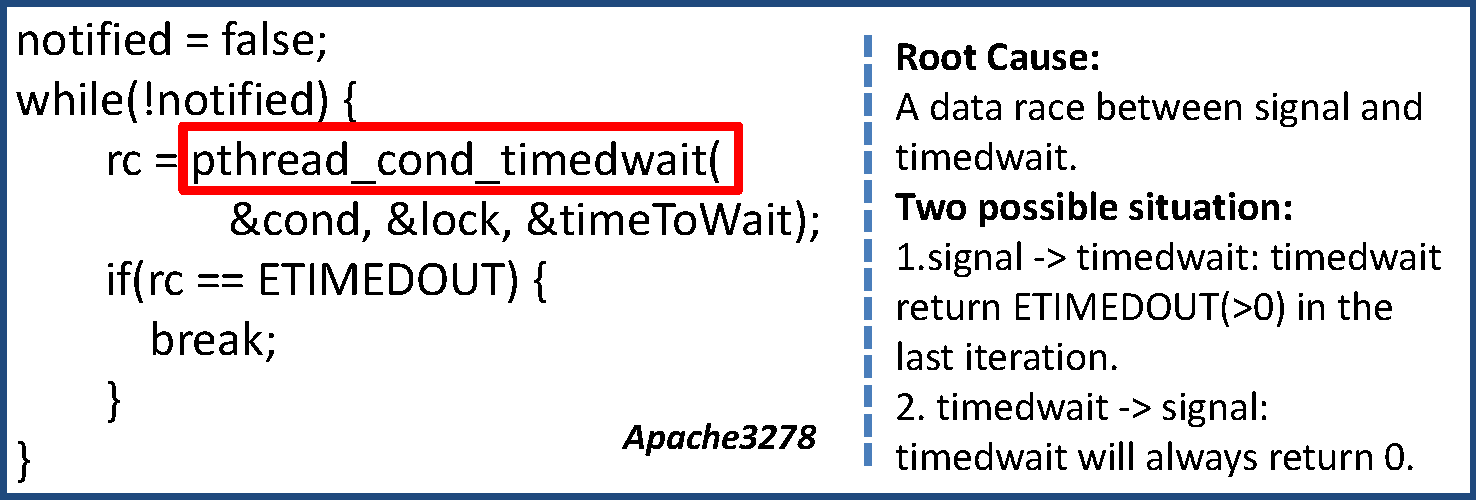
\includegraphics[width=3in]{figures/Apache3278}
\caption{An Apache bug diagnosed by Return}
\label{fig:Apache3278}
\end{center}
\end{figure}
}

\begin{figure}
\centering
\lstinputlisting[basicstyle=\ttfamily\footnotesize,numbers=left]{figures/Apache3278.c}
\caption{An Apache bug diagnosed by Return}
\label{fig:Apache3278}
\end{figure}

\comment{
\begin{figure}
\begin{center}
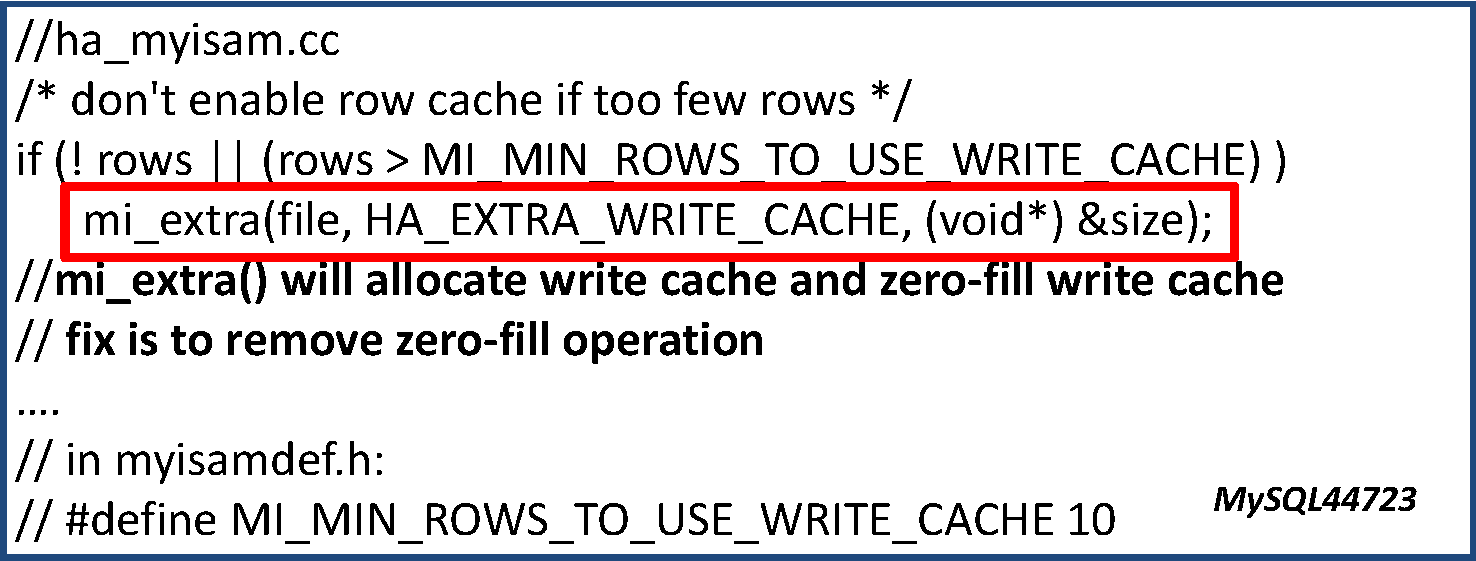
\includegraphics[width=3in]{figures/MySQL44723}
\caption{A MySQL bug diagnosed by Branch}
\label{fig:MySQL44723}
\end{center}
\end{figure}
}


\begin{figure}
\centering
\lstinputlisting[basicstyle=\ttfamily\footnotesize,numbers=left]{figures/MySQL44723.c}
\caption{A MySQL bug diagnosed by Branch}
\label{fig:MySQL44723}
\end{figure}

In most cases, the failure predictor
is very close to the final patch of the performance problem (within 10 lines
of code).
For example, the patch for the Apache bug in Figure 
\ref{fig:Apache3278} is only two lines away from the failure predictor.
As another example, 
the top-ranked failure predictor for the MySQL bug shown in 
Figure \ref{fig:MySQLintro} is at the \lstinline{if(!rows)} branch, and
the patch exactly changes that branch. 




There are also two cases, where the failure predictor is highly related to the
root cause but is in different files from the final patch.
For example, Figure~\ref{fig:MySQL44723} illustrates the performance problem
reported in MySQL\#44723.
MySQL44723 is caused by unnecessarily zero-filling the write cache. 
Users noticed that there is a huge performance difference between 
inserting 9 rows of data and 11 rows of data.
Our statistical debugging points out that the failure is highly
related to taking the
\texttt{(row > MI\_MIN\_ROWS\_TO\_USE\_WRITE\_CACHE)} branch.
That is, success runs never take this branch, yet failure runs always
take this branch.
This is related to the root cause --- an inefficient implementation
of function \texttt{mi\_extra}, and the patch makes \texttt{mi\_extra}
more efficient.

Note that identifying the correct failure predictor is not trivial.
As shown by the ``\# of candidate predicates'' column
of Table \ref{tab:in-house}, there is a large number of predicates that
have been observed true for at least once in failure runs.
Statistical debugging is able to identify the most failure predicting ones
out of thousands or even hundreds of thousands of candidate predicates.

\begin{table*}[tb!]
\begin{adjustwidth}{-.5in}{-.5in}
\small
\centering
{
\begin{tabular}{|lcccccc|}
\hline
&Apache&Chrome&GCC&Mozilla&MySQL&Total\\
\hline
Total \# of bugs  & 16 & 5 & 9 & 19 & 16 & 65 \\
\hline
\multicolumn{7}{|c|}{\bf \# of bugs the default CBI model can help}\\
\multicolumn{1}{|l}{{ Branches} }
&1&0&2&5&5&13\\
\multicolumn{1}{|l}{{ Returns} }
&1&0&0&0&1&2\\
\multicolumn{1}{|l}{{ Scalar-Pairs} }
 &0&0&0&0&0&0\\
\hline
\multicolumn{7}{|c|}{\bf \# of bugs $\Delta$LDA model can help}\\
\multicolumn{1}{|l}{{ Branches$_{\text{loop}}$} }
&10&4&7&12&10&43\\
\multicolumn{1}{|l}{{ Returns} }
%\multicolumn{1}{|l}{{ Returns$>$Branches} }
&0 &0&0& 0&0&0\\
%\multicolumn{1}{|l}{{ Returns$==$Branches} }
%&9&2&4&5&5&25\\
%\multicolumn{1}{|l}{{ Returns$<$Branches} }
%&1&2&1&6&3&13\\
\multicolumn{1}{|l}{{ Scalar-Pairs} }
%\multicolumn{1}{|l}{{ Scalar-Pairs$>$Branches} }
&0 &0&0&0 &0&0\\
%\multicolumn{1}{|l}{{ Scalar-Pairs$==$Branches} }
%&9&4&4&12&9&38\\
%\multicolumn{1}{|l}{{ Scalar-Pairs$<$Branches} }
%&1&0&2&0&0&3\\
\hline
\multicolumn{7}{|c|}{\bf \# of bugs above designs cannot help}\\
\multicolumn{1}{|l}{{ } }
&4&1&0&2&0&7 \\
\hline
\end{tabular}
}
\end{adjustwidth}
\caption{How different predicates work for diagnosing user-reported performance bugs (In this manual inspection, if more than one 
predicate can help diagnose a problem, we only count the predicate
that is most directly related to the root cause)}
\label{tab:predicate}
\end{table*}

\paragraph{Comparing with the profiler}
For eight cases where the basic statistical model is useful, profilers fail miserably. 
In terms of identifying root causes (i.e., what causes the inefficient 
computation), among these 8 cases,
the root-cause functions are ranked from number 11 to 
number 1037 for 5 cases. In the other 3 cases, the
function that contains the root cause does not even appear in the profiling 
result list (i.e., these functions execute for such a short amount of time that
they are not even observed by profilers).

Even if we consider functions in the call stacks of top-ranked
profiler functions, profiler is helpful for only one out of these eight cases,
as shown by the ``Stack'' column of Table \ref{tab:in-house}. That is, for
MySQL44723, the root cause function is the caller's caller of the top ranked
function in profiler results. For the other seven benchmarks, the root
cause functions do not appear on the call stacks of the top five ranked 
functions in profile results.




In terms of suggesting fix strategies, profiler results provide no hint
about how to solve the performance problem. Instead, the statistical debugging
results are informative.
For example, among the 7 cases where branch predicates are 
best failure predictors, the fixes either directly change the branch condition 
(5 cases) or optimize the code in the body of the branch (2 cases).
For the one case where a return predicate is the best failure predictor,
the fix affects the return value of the corresponding function.


\subsubsection{Results for $\Delta$LDA model}
\label{sec:deltalda_results}


\input section/5_delta-lda




\subsection{Manual inspection}
\label{sec:manual_results}

In addition to the above experimental study, we also manually checked
which predicate, if any, would help diagnose each of the 65 user-reported
performance bugs in our benchmark set. The result is shown in 
Table~\ref{tab:predicate}. 

Assuming the basic statistical model,  
traditional predicates (i.e., branches, returns, and scalar-pairs) 
can diagnose 15 out of 65 performance 
problems. Among them,
branch predicates are the most helpful, able to diagnose 13 performance 
problems; return predicates can diagnose 2 performance problems; 
scalar-pair
predicates are the least useful among the three in our study.




Among the ones that cannot be diagnosed by the basic statistical model,
43 of them are caused by inefficient loops. We expect that the 
$\Delta$LDA statistical model can identify root-cause related branch predicates
(denoted as ``Branches$_{\text{loop}}$'' in Table~\ref{tab:predicate}).
That is, the loop-condition branch related to the loop that is executed for too
many times
during failure runs will be ranked high by the $\Delta$LDA model.
Some scalar-pair predicates and function-return predicates could also
help failure diagnosis under the $\Delta$LDA model. For example, the
loop-condition of an inefficient loop could involve the comparison between
two scalar variables; the inefficient loop could invoke a function that
happens to always return positive values; and so on. However, these predicates
will not provide more information than branch predicates. Therefore, we do
not mark them in Table \ref{tab:predicate}.

The remaining 7 performance problems are mostly caused by unnecessary I/Os
or other system calls, not related to any predicates discussed above.

\subsection{Discussion}

Putting our manual inspection results and
experimental evaluation results together, we conclude the following:

\begin{enumerate}
\item Statistical debugging can help the diagnosis of many
user-reported performance problems, improving the state of the art in 
performance diagnosis;

\item Two design points of statistical debugging are particularly useful
for diagnosing performance problems. They are branch predicates under
basic statistical model and branch predicates under $\Delta$LDA model.
These two design points complement each other, providing
\textbf{almost full} coverage of performance problems that we have studied;

\item The basic statistical model that works for most functional bugs
\cite{liblit03,liblit05,tarantula1,tarantula2,tarantula.darko,CCI,joy.asplos13}
is very useful for performance diagnosis too, but still leaves many performance
problems uncovered; statistical models that
consider the number of times a predicate is true 
in each run (e.g., the $\Delta$LDA model)
is needed for diagnosing performance problems.

\item Statistical debugging alone cannot solve all the problem
of diagnosing performance problems. Although statistical debugging
can almost always provide useful information for performance diagnosis, 
developers still
need help to figure out the final patches. Especially, when an inefficient
loop is pointed out by the $\Delta$LDA model, 
developers need more program analysis to understand why the loop is inefficient
and how to optimize it.
\end{enumerate}



To guide future research on performance diagnosis, we further
studied those 43 loop-related performance problems, and manually categorized 
their fix strategies, as shown in
Table \ref{tab:loop-rootcause}.
We expect future performance diagnosis systems to use static or
dynamic analysis to automatically figure out the detailed 
root causes, differentiate effects from causes, and suggest
detailed fix strategies, after statistical debugging identifies
root-cause loop candidates.


%%%%%%%%%%%%%%%%%%%COMMENT OUT%%%%%%%%%%
\comment{
\begin{table*}[tb!]
\begin{adjustwidth}{-.5in}{-.5in}
\small
\centering
{
\begin{tabular}{|c|c|c|c|c|c|c|}
\hline
\multicolumn{1}{|c|}{Predicates} &Apache&Chrome&GCC&Mozilla&MySQL&Total\\
\hline
Total \# of bugs    & 16 & 5 & 9 & 19 & 16 & 65 \\
\hline

Branches                  &1&0&2&5&5&13\\
Returns                  &1&0&0&0&2&3\\
Scalar-Pairs             &0&0&0&0&0&0\\
Loop                    &10&4&7&12&9&42\\
Others                  &4&1&0&2&0&7\\
\hline
\end{tabular}
}
\end{adjustwidth}
\caption{How different predicates work for diagnosing user-perceived performance bugs (manual inspection)}
\label{tab:predicate}
\end{table*}
}

\comment{
\begin{figure}[h!]
\centering
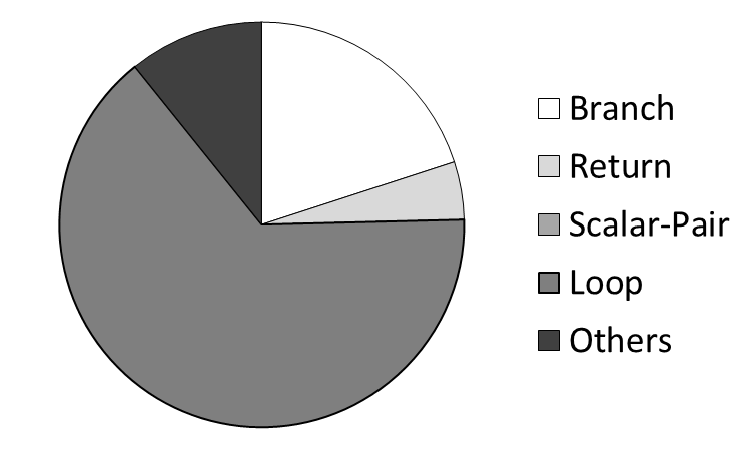
\includegraphics[width=2.5in]{figures/pie}
\caption{How different predicates work for diagnosing user-perceived performance bugs (manual inspection)}
\label{fig:predicate}
\end{figure}
}

\section{Production-run statistical debugging}
\label{sec:lbr}
In-house performance diagnosis discussed in Section \ref{sec:inhouse} assumes
that users file a detailed bug report and developers can repeat the 
performance problem at the development site. Unfortunately, this does not always
happen. In many cases, production-run users only send 
back a simple automatically generated report, claiming that a failure has 
happened, together with a small amount
of automatically collected run-time information. 

The key challenge of diagnosing production-run failures is how to satisfy the
following three requirements simultaneously:

\begin{enumerate}
\item Low run-time overhead. 
The diagnosis tool will not be accepted by end users, if it incurs too much
slow down to each production run.

\item High diagnosis capability. 
The diagnosis tool is useful to developers only when it can accurately 
provide failure root cause information.

\item Short diagnosis latency. 
Short diagnosis latency can speed up patch design and improve system
availability.
\end{enumerate}

This section discusses this issue
in the context of performance bugs.

\subsection{Design}
The state of the art on production-run
functional bug diagnosis \citep{liblit03,liblit05,CCI,joy.asplos13} proposes
to satisfy the first two requirements (i.e., low overhead and high capability)
by combining  
\textit{sampling} techniques with
statistical debugging.
By randomly sampling predicates at run time, the overhead can be lowered;
by processing predicates collected from many failure and success runs
together, the diagnosis capability can be maintained for the diagnosis of most
functional bugs \citep{liblit03,liblit05,CCI,joy.asplos13}.
The only limitation is that sampling could affect diagnosis latency 
--- the same failure needs to occur for many times until sufficient information
can be sampled. This is especially a problem for software that is not widely
deployed and bugs that do not manifest frequently.
We plan to follow this approach and apply it for production-run performance
diagnosis.

Different from production-run functional failure diagnosis
\citep{liblit03,liblit05,CCI,joy.asplos13}, production-run performance diagnosis
needs to have a slightly different failure-reporting process.
Traditional functional failure diagnosis assumes that a profile of
sampled predicates will be collected after
every run. This profile will be marked as
\textit{failure} when software encounters typical failure symptoms such as 
crashes, error messages, and so on; the profile will be marked
as \textit{success} otherwise. The same process does not apply to performance
failures, because most performance failures are observed through
comparisons across runs, as discussed in Section \ref{sec:study}. 

To adapt to the unique way that performance problems are observed, we 
expect that users will explicitly mark a profile as \textit{success}, 
\textit{failure}, or \textit{do-not-care} (the default marking), when they 
participate in production-run performance diagnosis. For most performance 
problems (i.e., those problems observed through comparisons), do-not-care
profiles will be ignored during statistical debugging. For performance problems
that have non-comparison-based symptoms (i.e. application freeze), all
profiles collected from production runs will be considered during statistical
debugging.

One issue not considered in this paper is \textit{failure bucketing}. That is, 
how to separate failure (or success) profiles related to different software 
defects. This problem is already handled by some statistical models 
\citep{liblit03,liblit05} that can discover multiple failure predictors
corresponding to different root causes mixed in one
profile pool, as well as some failure bucketing techniques
\citep{hunt.sosp09}
that can roughly cluster profiles based on likely root causes.
Of course, performance diagnosis may bring new challenges to these
existing techniques. We leave this for future research.

\subsection{Experimental evaluation}

Our evaluation will aim to answer two key questions:

\begin{enumerate}
\item Can sampling lower the overhead and maintain the capability of
performance-related statistical debugging? A positive answer would indicate
a promising approach to production-run performance diagnosis.

\item What is the impact of sampling to diagnosis latency?
Traditionally, if we use 1 out of 100 sampling rate, we need hundreds of failure
runs to achieve good diagnosis results. Since many performance bugs lead
to repeated occurrences of an event at run time, it is possible that fewer
failure runs would be sufficient for performance diagnosis. If this heuristic
is confirmed, we will have much shorter diagnosis latency than traditional
sampling-based failure diagnosis for functional bugs.
\end{enumerate}


\subsubsection{Methodology}
\paragraph{Benchmarks and inputs}
We reuse the same set of benchmarks shown in Table~\ref{tab:app_bug}. 
We also use the same methodology to generate inputs and drive success/failure
runs. The only difference is that for the four performance problems that users
do not report any good inputs, we will use completely random inputs to produce
success-run profiles.

\paragraph{Tool implementation}
To sample return predicates, we directly use CBI \cite{liblit03,liblit05}.
CBI instruments program source code to conduct sampling.
Specifically, CBI instrumentation keeps a global countdown to decide how many 
predicates can be skipped before next sample. 
When a predicate is sampled, 
the global countdown is reset to a new value based on a geometric distribution 
whose mean value is the inverse of the sampling rate. 

To sample branch predicates, we directly use CBI for benchmarks written in 
C. For all MySQL and some Mozilla benchmarks that are written in C++, since
CBI does not work for C++ code, we conduct sampling through
hardware performance counters following the
methodology described in previous work \cite{joy.asplos13}.
Specifically, hardware performance
counters are configured so that an interrupt will be triggered every $N$
occurrences of a particular performance event (e.g, branch-taken event), with no changes to the program.

\paragraph{Metrics and settings}
We will evaluate all three key metrics for failure diagnosis:
(1) run-time overhead, measured by the slow down caused by information
collection at every run;
(2) diagnosis capability,
measured by whether top ranked failure predictors are 
related to failure root causes, as discussed in 
Section~\ref{sec:inhouse_results}.
(3) diagnosis latency,
measured by how many failure runs are needed 
to complete the diagnosis. 

By default, we keep the sampling rate at roughly
1 out of 10000
and use samples
collected from 1000 failure runs and 1000 success runs for failure diagnosis. 

In addition to experiments under the default setting, we also evaluate the 
impact of different numbers of failure/success runs, ranging from 10 to 1000,
while keeping the sampling rate fixed, and evaluate the impact of different
sampling rates, ranging from roughly 1 out of 100 to roughly 1 out of 100000,
while keeping the number of failure/success runs fixed.
Particularly, we will try using only 10 success runs
and 10 failure runs, under the default sampling rate, to see if we can achieve 
good diagnosis capability,
low diagnosis latency, and low run-time overhead \emph{simultaneously}. 

Since sampling is random, we have repeated our evaluation for several rounds to confirm that all
the presented results are stable.

For every performance problem benchmark, the results presented below are 
obtained under the
combination of predicate and statistical model that is shown to be (most) 
effective
in Table \ref{tab:in-house} (Section \ref{sec:inhouse}).
That is, basic model plus branch predicates are used for seven benchmarks;
basic model plus return predicates are used for one benchmark;
$\Delta$LDA model plus branch$_{\text{loop}}$ predicates are used for the remaining twelve  
benchmarks, including GCC12322.
Since sampling can only lower overhead and cannot
improve the diagnosis capability, those combinations that fail to deliver
useful diagnosis results in Table \ref{tab:in-house} still fail to deliver
useful diagnosis results in our sampling-based evaluation.

\subsubsection{Results}

\begin{table}[h!]
  \centering
  \small
  \newcommand{\Yes}[1]{\checkmark{}$_#1$}
  \newcommand{\No}[0]{-}
  \begin{tabular}{lccccc}
    \toprule     
   {\bf BugID}             &  \multicolumn{4}{c}{ Diagnosis Capability}   & Overhead \\
                           
    \cmidrule(lr){2-5}
    (\# of runs)                 &  (10)     &   (100)    &    (500)    & (1000)     &   per run\\
    \midrule 

    Mozilla258793                & \No       & \Yes{1}    &  \Yes{1}    & \Yes{1}    &   2.39\%        \\
    Mozilla299742                & \No       & \No        &  \Yes{1}    & \Yes{1}    &   4.27\%        \\
    Mozilla347306                & \Yes{1}   & \Yes{1}    &  \Yes{1}    & \Yes{1}    &   1.42\%  \\
    Mozilla416628                & \Yes{1}   & \Yes{1}    &  \Yes{1}    & \Yes{1}    &   2.03\%   \\
    \midrule
    MySQL15811                   & \Yes{1}   & \Yes{1}    & \Yes{1}     & \Yes{1}    &  2.25\% \\
    MySQL26527                   & \No       & \No        & \Yes{1}     & \Yes{1}    &  6.05\% \\
    MySQL27287                   & \Yes{1}   & \Yes{1}    & \Yes{1}     & \Yes{1}    &  3.02\% \\
    MySQL40337                   & \No       & \Yes{1}    & \Yes{1}     & \Yes{1}    &  2.69\% \\
    MySQL42649                   & \No       & \No        & \Yes{2}     & \Yes{1}    &  6.10\% \\
    MySQL44723                   & \No       & \Yes{1}    & \Yes{1}     & \Yes{1}    &  3.16\% \\
    \midrule
    Apache3278                   & \No       & \No        &  \No        & \No        &  0.23\%         \\
    Apache34464                  & \Yes{3}   & \Yes{3}    & \Yes{3}     & \Yes{3}    &  0.18\%     \\
    Apache47223                  & \Yes{1}   & \Yes{1}    & \Yes{1}     & \Yes{1}    &  0.13\%         \\
    Apache32546                  & \Yes{1}   & \Yes{1}    & \Yes{1}     & \Yes{1}    &  0.38\%     \\
    \midrule
    GCC1687                      & \Yes{1}   & \Yes{1}    &  \Yes{1}    & \Yes{1}    &  0.80\%  \\
    GCC8805                      & \Yes{4}   & \Yes{4}    &  \Yes{4}    & \Yes{4}    &  1.81\%  \\
    GCC15209                     & \No       & \No        &  \Yes{1}    & \Yes{1}    &  2.37\%        \\
    GCC21430                     & \Yes{1}   & \Yes{1}    &  \Yes{1}    & \Yes{1}    &  7.55\%  \\
    GCC46401                     & \Yes{2}   & \Yes{2}    &  \Yes{2}    & \Yes{2}    &  2.91\%  \\
    GCC12322                     & \No       & \No        &  \No        & \No        &  2.33\%  \\

    \bottomrule
   \end{tabular}
  \nocaptionrule
  \caption{Run-time overhead and diagnosis capability evaluated with the default sampling rate (1 out of 10000); 10, 100, 500, 1000 represents the different numbers of success/failure runs used for diagnosis.}
  \label{tab:LBR}
\end{table}



\begin{table*}
  \centering
  \footnotesize
  \newcommand{\Yes}[1]{\checkmark{}$_#1$}
  \newcommand{\No}[0]{-}
  \begin{tabular}{lcccccccccccc}
    \toprule     
   {\bf BugID} & \multicolumn{4}{c}{ Diagnosis Capability} &\multicolumn{4}{c}{Overhead} & \multicolumn{4}{c}{Avg. \# of sampled predicates} \\
                           
    \cmidrule(lr){2-5}
    \cmidrule(lr){6-9}
    \cmidrule(lr){10-13}
    (sampling rate)  &($\frac{1}{10^2}$)&($\frac{1}{10^3}$)&($\frac{1}{10^4}$)& ($\frac{1}{10^5}$)  &($\frac{1}{10^2}$) &($\frac{1}{10^3}$)&($\frac{1}{10^4}$)  & ($\frac{1}{10^5}$)  & ($\frac{1}{10^2}$)  & ($\frac{1}{10^3}$)    & ($\frac{1}{10^4}$)   &  ($\frac{1}{10^5}$)         \\
    \midrule 

    Mozilla258793    &  *    & \Yes{1}  & \Yes{1}   & \Yes{1}     & *       & 24.36\% &  2.39\%     &  1.84\%     & *         & $1.42*10^6$   & $1.45*10^5$   &  $1.49*10^4$           \\
    Mozilla299742    &  *    & \Yes{1}  & \Yes{1}   & \Yes{2}     & *       & 30.84\% &  4.27\%     &  4.16\%     & *         & $1.87*10^5$   & $1.77*10^4$   &  $1.82*10^3$\\
    Mozilla347306    & \Yes{1} & \Yes{1}  & \Yes{1}   & \Yes{1}     & 69.73\%   & 8.27\%  &  1.42\%     &  0.56\%     &$7.13*10^6$  & $7.13*10^5$   & $7.13*10^4$   &  $7.13*10^3$\\
    Mozilla411722    & \Yes{1} & \Yes{1}  & \Yes{1}   & \Yes{1}     & 24.64\%   & 4.31\%  &  2.03\%     &  1.36\%     &$8.18*10^5$  & $8.18*10^4$   & $8.17*10^3$   &  816.56  \\
    \midrule
    MySQL15811       & *     & \Yes{1}  & \Yes{1}   & \Yes{1}     & *       & 7.65\%  &  2.25\%     &  1.53\%     & *         &$3.67*10^5$    &  $1.67*10^5$  & $1.66*10^4$          \\
    MySQL26527       & *     & \Yes{1}  & \Yes{1}   & \No         & *       & 6.40\%  &  6.05\%     &  4.53\%     & *         &$3.23*10^3$    &  921.41       & 92.60 \\
    MySQL27287       & *     & \Yes{1}  & \Yes{1}   & \Yes{1}     & *       & 4.63\%  &  3.02\%     &  0.61\%     & *         &$2.52*10^6$    &  $1.15*10^6$  & $1.19*10^5$\\
    MySQL40337       & *     & \Yes{1}  & \Yes{1}   & \No         & *       & 10.88\% &  2.69\%     &  2.28\%     & *         &$5.10*10^6$    &  $1.66*10^6$  & $1.42*10^5$\\
    MySQL42649       & *     & \Yes{1}  & \Yes{1}   & \No         & *       & 8.28\%  &  6.10\%     &  3.93\%     & *         &$7.25*10^3$    &  $1.14*10^3$  &  128.53\\
    MySQL44723       & *     & \Yes{1}  & \Yes{1}   & \Yes{1}     & *       & 7.10\%  &  3.16\%     &  2.24\%     & *         &$3.23*10^5$    &  $1.83*10^5$  & $1.46*10^4$\\
    \midrule
    Apache3278       & \Yes{1} & \No      & \No       & \No         & 0.23\%    & 0.23\%  &   0.23\%    &  0.23\%     & 0.21        & 0.01          & 0             & 0\\
    Apache34464      & \Yes{3} & \Yes{3}  & \Yes{3}   & \Yes{3}     & 29.45\%   & 2.62\%  &   0.18\%    &  0.04\%     & $2.50*10^7$ &$2.50*10^6$    & $2.49*10^5$   &$2.50*10^4$\\
    Apache47223      & \Yes{1} & \Yes{1}  & \Yes{1}   & \Yes{1}     & 12.58\%   & 1.28\%  &   0.13\%    &  0.12\%     & $6.27*10^6$ &$6.26*10^5$    & $6.27*10^4$   &$6.27*10^3$\\
    Apache32546      & \Yes{1} & \Yes{1}  & \Yes{1}   & \Yes{1}     & 0.24\%    & 0.39\%  &   0.38\%    &  0.40\%     & $9.75*10^3$ &977.72         & 99.01         &9.5\\
    \midrule
    GCC1687          & \Yes{1} & \Yes{1}  & \Yes{1}   & \Yes{1}     & 47.30\%   & 5.34\%  &  0.80\%     &   0.43\%    & $3.18*10^7$ &$3.18*10^6$    & $3.18*10^5$   &$3.17*10^4$\\
    GCC8805          & \Yes{4} & \Yes{4}  & \Yes{4}   & \Yes{4}     & 50.92\%   & 7.33\%  &  1.81\%     &   1.05\%    & $1.63*10^7$ &$1.63*10^6$    & $1.63*10^5$   &$1.63*10^4$\\
    GCC15209         & \Yes{1} & \Yes{2}  & \Yes{1}   & \Yes{2}     & 41.06\%   & 8.43\%  &  2.37\%     &   1.27\%    & $3.35*10^4$ &$3.35*10^3$    & 334.72        &33.64\\
    GCC21430         & \Yes{1} & \Yes{1}  & \Yes{1}   & \Yes{1}     & 64.98\%   & 13.68\% &  7.55\%     &   5.07\%    & $9.15*10^7$ &$9.15*10^6$    & $9.15*10^5$   &$9.15*10^4$\\
    GCC46401         & \Yes{2} & \Yes{2}  & \Yes{2}   & \Yes{2}     & 88.97\%   & 13.04\% &  2.91\%     &   0.46\%    & $8.88*10^7$ &$8.88*10^6$    & $8.88*10^5$   &$8.88*10^4$\\
    GCC12322         & \No     & \No      & \No       & \No         & 15.55\%   & 2.33\%  &  2.33\%     &   0.56\%    & $9.97*10^7$ &$9.97*10^6$    & $9.97*10^5$   &$9.97*10^4$\\

    \bottomrule
   \end{tabular}
  \nocaptionrule
  \caption{Diagnosis capability, overhead, and average number of samples in each run under different sampling rates by using 1000 success/failure runs 
  (*: no results are available, because
   hardware-based sampling cannot be as frequent as $1/100$ and software-based
   CBI sampling does not apply for these C++ benchmarks.
   )}
  \label{tab:rate}
\end{table*}


\paragraph{Run-time overhead}
As shown in Table \ref{tab:LBR}, the run-time overhead is small
under the default sampling rate (i.e., 1 out of 10000).
It is below 5\% in all but three cases, and is always below 8\%.

As expected, the overhead is sensitive with the sampling rate. As shown in
Table~\ref{tab:rate}, it can be further lowered to be mostly below 2\% under
the $\frac{1}{10^{5}}$ sampling rate, and could be as large as over 40\% under
the $\frac{1}{100}$ sampling rate.


\paragraph{Diagnosis capability}
As shown by Table \ref{tab:LBR}, with 1000 success runs
and 1000 failure runs, sampling did very little damage to
the diagnosis capability of statistical debugging. 
Apache\#3278 is the only one, among all benchmarks, where 
failure diagnosis fails under this sampling setting.
For all other benchmarks, the
rankings of the ideal failure predictors remain the same as those 
without sampling in Table \ref{tab:in-house}.

Also as expected, the diagnosis capability would decrease under sparser
sampling or fewer failure/success runs. As shown in Table \ref{tab:rate},
under the default setting of 1000 success/failure runs, the diagnosis capability
is roughly the same between $\frac{1}{10^{3}}$ sampling rate and 
$\frac{1}{10^{4}}$ sampling
rate, but would drop with $\frac{1}{10^{5}}$ sampling rate. 
Four benchmarks that can be diagnosed 
with more frequent sampling cannot be diagnosed with
$\frac{1}{10^{5}}$ sampling rate.
Clearly, more
runs will be needed to restore the diagnosis capability with a lower
sampling rate.

\paragraph{Diagnosis latency}
Diagnosis latency versus run-time overhead and diagnosis capability 
is a fundamental trade-off facing
sampling-based statistical debugging for functional bugs \cite{liblit03,liblit05,CCI}.
With sampling, intuitively, more failure runs are needed
to collect sufficient diagnosis information. This is \textbf{not} a problem for widely
deployed software projects. In those projects, the same failure tends to quickly occur
for many times on many users' machines
\cite{hunt.sosp09}. However, this is a problem
for software that is not widely deployed.

We quantitatively measured the impact of sampling to diagnosis latency in 
Table \ref{tab:LBR}. As we can see, three benchmarks need about 100 failure
runs for their sampling-based diagnosis to produce useful results; 
four benchmarks need about 500 failure runs; and one benchmark, Apache\#3278, 
needs more than 1000 failure runs. This
indicates longer diagnosis latencies than the non-sampling-based diagnosis
evaluated in Section \ref{sec:inhouse}, where only 10 failure runs are used.

Interestingly, there are 11 benchmarks, whose diagnosis latency is \textbf{not}
lengthened by sampling. As shown in Table \ref{tab:LBR}, even with only
10 failure runs, the sampling-based diagnosis still produces good failure
predictors. These are exactly all the 11 benchmarks that $\Delta$LDA model 
suits in Table \ref{tab:in-house}. 
For all these benchmarks,
the rankings are exactly the same with or without
sampling, with just 10 failure runs. Consequently, sampling
allows us to achieve low run-time overhead ($<$10\%), high diagnosis capability,
and low diagnosis latency \textbf{simultaneously}, a feat that is almost 
impossible
for sampling based functional bug diagnosis.
%TODO linhai please check if liblit's work did some experiments on this.

The nice results for these 11 benchmarks can be explained by a unique feature
of performance bugs, especially loop-related
performance bugs --- their root-cause related predicates are often evaluated to 
be true for many times in one run, which is why the performance is poor.
Consequently, even under sparse sampling, there is still a high chance that the
root-cause related predicates can be sampled, and be sampled more frequently
than root-cause unrelated predicates.


Finally, even for the other 9 benchmarks, 
$\frac{1}{10^4}$ sampling rate does not 
extend diagnosis
latency by $10^4$ times. In fact, for most of these benchmarks, 100 -- 500
failure runs are sufficient for failure diagnosis under 
$\frac{1}{10^4}$ sampling
rate. Our investigation shows that the root-cause code regions in these 
benchmarks
are all executed for several times during the user-reported failure runs, 
which
is likely part of the reason why users perceived the performance problems. 
Consequently, the negative impact of sampling on diagnosis latency is
alleviated.

\comment{
\begin{table}[h!]
  \centering
  \small
  \newcommand{\Yes}[1]{\checkmark{}$_#1$}
  \newcommand{\No}[0]{-}
  \begin{tabular}{lccc}
    \toprule     
   {\bf BugID} & \multicolumn{3}{c}{Sampling Rate} \\
                           
   \cmidrule(lr){2-4}

                        &  1/10 & 1/100 & 1/1000                     \\
    \midrule 

    Mozilla258793       & \Yes{1}    &  \Yes{1}      &  \Yes{1}    \\
    Mozilla299742       & \Yes{1}    &  \Yes{1}      &  \Yes{2}       \\
    Mozilla347306       & \Yes{1}    &  \Yes{1}      &  \Yes{1}      \\
    Mozilla416628       & \Yes{1}    &  \Yes{1}      &  \Yes{1}       \\
    \midrule
    MySQL15811          &  \Yes{1}   &  \Yes{1}      &  \Yes{1}      \\
    MySQL26527          &  \Yes{1}   &  \Yes{1}      &  \No      \\
    MySQL27287          &  \Yes{1}   &  \Yes{1}      &  \Yes{1}       \\
    MySQL40337          &            &     &        \\
    MySQL42649          &  \Yes{1}   &  \Yes{1}      &  \No        \\
    MySQL44723          &  \Yes{1}   &  \Yes{1}      &  \Yes{1}       \\
    \midrule
    Apache3278          & \Yes{1}    &  \Yes{1}      &   \No    \\
    Apache34464         & \Yes{1}    &  \Yes{1}      &   \Yes{1}    \\
    Apache47223         & \Yes{1}    &  \Yes{1}      &   \Yes{1}     \\
    Apache32546         & \Yes{1}    &  \Yes{1}      &   \Yes{1}     \\
    \midrule
    GCC1687             & \Yes{1}    &  \Yes{1}      &   \Yes{1}      \\
    GCC8805             & \No        &  \No          &   \No       \\
    GCC15209            & \Yes{1}    &  \Yes{1}      &   \Yes{1}      \\
    GCC21430            & \Yes{1}    &  \Yes{1}      &   \Yes{1}     \\
    GCC46401            & \Yes{2}    &  \Yes{2}      &   \Yes{2}     \\
    GCC12322            &     &     &        \\

    \bottomrule
   \end{tabular}
  \nocaptionrule
  \caption{Diagnosis capability under different sampling rates}
  \label{tab:rate}
\end{table}
}




\section{Related Work}

\subsection{Empirical study of performance bugs}
Recently, several empirical studies have been conducted for real-world
performance bugs. They all have different focuses.
Some of them \cite{Zaman2012MSR} compare the
qualitative difference between performance bugs and non-performance bugs 
across impact, context, fix and fix validation; some of them
\cite{PerfBug} look at 
how performance bugs are introduced, 
how performance bugs manifest, 
and how performance bugs are fixed; 
some of them
\cite{SmartphoneStudy} focuses on performance bugs in smart-phone applications.
Different from all previous studies, our study aims to provide guidance
to performance problem diagnosis, and hence focuses on how performance
problems are noticed and reported by end users. 

A most recent study conducted by Nistor et al. \cite{Nistor2013MSR} is similar
with our bug characteristics study (Section \ref{sec:study}) 
in that it also finds that performance problems take long time
to get diagnosed and the help from profilers is very limited. However, the
similarity ends here. Different from
our study, this recent work did not study how performance problems are
observed and reported by end users. Its bug set includes many problems
that are not perceived by end users and are instead discovered through 
developers' code inspection, which is not the focus of our study. In short,
it does not aim to guide automated diagnosis of performance problems, 
and is hence different
from our work.

\subsection{Performance problem diagnosis}
Diagnosis tools aim to identify root causes and suggest fix strategies when 
software failures happen. Tools have been proposed to diagnose certain
type of performance problems.

X-ray~\cite{Attariyan:2012:XAR:2387880.2387910} aims to diagnose performance 
problems caused by end users. The root causes discussed in the X-ray paper are 
unexpected inputs or configurations that can be changed by end users. 
X-ray pin-points the inputs or configuration entries that are most 
responsible for a performance problem, and help users to solve the 
performance issues by themselves (by changing the inputs or configuration
entries). 
The main technique used in X-ray is called performance summarization, which 
first attributes a performance 
cost to each basic block, and then estimates the possibility that each block 
will be executed 
due to certain input entry, and finally ranks all input entries.
Techniques discussed in our paper aim to help developers. We want to provide 
information to help developers change inefficient code and fix performance bugs.
IntroPerf~\cite{IntroPerf} automatically infers the latency of user-level and
kernel-level function calls based on operating system tracers.
StackMine~\cite{Han:2012:PDL:2337223.2337241} automatically identifies certain
call-stack patterns that are correlated with performance problems of 
event handlers.
\citet{TaoAsplos2014} automatically processes detailed system traces to 
help developers understand how performance impact propagates across system
components, and what are the performance causality relationships among
components and functions.
All these diagnosis tools are very useful in practice, but have different
focus from our work. They
do not aim to identify source-code fine-granularity 
root causes of performance problems reported by end users.

Many techniques been proposed to diagnose 
performance problems in distributed systems
\cite{Sambasivan:2011:DPC:1972457.1972463,Fonseca:2010:ETC:1863133.1863143,Kasick:2010:BPD:1855511.1855515,Xu:2009:DLS:1629575.1629587,aguilera03}.
These techniques often focus on identifying the faulty components/nodes or 
faulty interactions that lead to performance problems, which are different from our work.

\subsection{Performance bug detection}
Many performance bug detection tools have been proposed recently.
They each aims to find a specific type of hidden
performance bugs before the bugs lead to performance problems observed by
end users.

Some tools~\cite{Dufour:2008:STC:1453101.1453111, Xu:2009:GFP:1542476.1542523, Xu:2010:DIC:1806596.1806616}
detect runtime bloat, a common performance problem in object-oriented 
applications.
\citet{Xu:2010:FLD:1806596.1806617} targets 
low-utility data structures with unbalanced costs and benefits.
\citet{PerfBug} employ rule-based methods to detect performance bugs that
violate efficiency rules that have been violated before.
\citet{ORMPatterns} detect database related performance anti-patterns,
like fetching excessive data from database and issuing queries that could have
been aggregated.
WAIT~\cite{Altman:2010:PAI:1869459.1869519} focuses on bugs that
block the application from making progress.
\citet{Liu:2011:SPD:2048066.2048070} build two tools to attack the false 
sharing problem in multi-threaded software.
There are also tools that detect inefficient nested loops \cite{Alabama}
and workload-dependent
loops \cite{xiao13:context}.
%\citet{RegressCauses} discover performance regression using hardware
%counters and machine learning methods, and propose
%code change patterns that are likely responsible for the 
%discovered performance regression.

These bug-detection tools have different focus from our work. 
They do not focus on diagnosing general performance problems reported by 
end users. Most of them are also not 
guided by performance symptoms.

%\subsection{Profilers}
%Profilers are widely used by developers to diagnose performance problems. 
%For example, gprof~\cite{gprof} and oprofile~\cite{oprofile} are both
%widely used profilers.
%To use gprof, programs need to be compiled by using ``-pg'' option. 
%For each function call, gprof will record its caller. For each function, 
%gprof will record how many times it is called. 
%At run time, gprof will look at program counter each 0.01 second to record 
%which function is executing. 
%gprof provides two types of profiling results: 
%flat profile, which will rank each function based on how much time spent in 
%them, 
%and call graph, which shows how much time is spent in each function and their 
%children. 

%Oprofile does not instrument programs. 
%Oprofile asks users to specify hardware events and sampling frequency. 
%Every time the specified number of events occur, oprofile will record program counter value and call stack. 
%Similar to gprof, oprofile can also provide flat profile and call graph information. 

\section{Conclusion}
\label{sec:con}
Software design and implementation defects lead to not only functional 
misbehavior but also performance losses. Diagnosing performance problems
caused by software defects are both important and challenging. This paper 
made several contributions to improving the state of the art of diagnosing
real-world performance problems. Our empirical study showed that end users
often use comparison-based methods to observe and report performance problems,
making statistical debugging a promising choice for performance diagnosis. 
Our investigation of different design points of statistical debugging shows
that branch predicates, with the help of two types of statistical models, are  
especially helpful for performance diagnosis. It points out useful failure
predictors for 19 out of 20 real-world performance problems. 
Furthermore, our investigation shows that statistical debugging can also
work for production-run performance diagnosis with sampling support, incurring 
less than 10\% overhead in our evaluation. Our study also points out
directions for future work on fine-granularity performance diagnosis.


\acks
We thank the anonymous reviewers for their valuable comments which have substantially improved the content and presentation of this paper; 
Professor Darko Marinov and Professor Ben Liblit for their insightful feedback and help; Jie Liu for his tremendous help in statistical concepts and methods.
This work is supported in part by NSF grants CCF-1018180,
CCF-1054616, and CCF-1217582; and a Clare Boothe Luce
faculty fellowship.
  



%%\balance
%\begin{spacing}{0.65}

\balance
{
\bibliographystyle{abbrvnat}
\bibliography{debug,perf} 
}
%\end{spacing}
\end{document}


\lstset{
  basicstyle=\tiny,
  columns=fullflexible,
  numbersep=5pt,
  numberstyle=\scriptsize,
  showstringspaces=false,
  escapeinside={/*@}{@*/},
  belowcaptionskip=1\baselineskip,
  language=C,
  showstringspaces=false,
  keywordstyle=\bfseries,
  commentstyle=\itshape,
}

\tikzset{%
  node distance=1em,
  >=stealth,
  cfg/.style={%
    minimum width=2em,
    minimum height=1em,
    rounded corners=2pt,
    draw=black,
  },
  protected/.style={%
    cfg,
    fill=black!20,
  },
  ghost/.style={%
    minimum width=0,
    minimum height=0,
    shape=coordinate,
  },
  mutex/.style={
    midway,
  },
}

\urlstyle{sf}

\pdfpagewidth=8.5in
\pdfpageheight=11in

% Local variables:
% TeX-PDF-mode: t
% TeX-master: t
% End:

% LocalWords:  Crug cci
